% Copyright 2004 by Till Tantau <tantau@users.sourceforge.net>.
%
% In principle, this file can be redistributed and/or modified under
% the terms of the GNU Public License, version 2.
%
% However, this file is supposed to be a template to be modified
% for your own needs. For this reason, if you use this file as a
% template and not specifically distribute it as part of a another
% package/program, I grant the extra permission to freely copy and
% modify this file as you see fit and even to delete this copyright
% notice. 

\documentclass{beamer}

% There are many different themes available for Beamer. A comprehensive
% list with examples is given here:
% http://deic.uab.es/~iblanes/beamer_gallery/index_by_theme.html
% You can uncomment the themes below if you would like to use a different
% one:
%\usetheme{AnnArbor}
%\usetheme{Antibes}
%\usetheme{Bergen}
%\usetheme{Berkeley}
%\usetheme{Berlin}
%\usetheme{Boadilla}
%\usetheme{boxes}
%\usetheme{CambridgeUS}
%\usetheme{Copenhagen}
%\usetheme{Darmstadt}
%\usetheme{default}
%\usetheme{Frankfurt}
%\usetheme{Goettingen}
%\usetheme{Hannover}
%\usetheme{Ilmenau}
%\usetheme{JuanLesPins}
%\usetheme{Luebeck}
\usetheme{Madrid}
%\usetheme{Malmoe}
%\usetheme{Marburg}
%\usetheme{Montpellier}
%\usetheme{PaloAlto}
%\usetheme{Pittsburgh}
%\usetheme{Rochester}
%\usetheme{Singapore}
%\usetheme{Szeged}
%\usetheme{Warsaw}
\usepackage[3D]{movie15}
\usepackage{cancel}

\title{twoPhaseEulerNDPBMFoam}

% A subtitle is optional and this may be deleted
%\subtitle{OpenFOAM solver CFD_PBM}

\author{Ehsan Askari}
% - Give the names in the same order as the appear in the paper.
% - Use the \inst{?} command only if the authors have different
%   affiliation.

\institute[Universities of Sherbrooke] % (optional, but mostly needed)
{
  
  Department of Chemical Engineering\\
  University of Sherbrooke
}
% - Use the \inst command only if there are several affiliations.
% - Keep it simple, no one is interested in your street address.

\date{Group meeting, March 2016}
% - Either use conference name or its abbreviation.
% - Not really informative to the audience, more for people (including
%   yourself) who are reading the slides online

%\subject{Theoretical Computer Science}
% This is only inserted into the PDF information catalog. Can be left
% out. 

% If you have a file called "university-logo-filename.xxx", where xxx
% is a graphic format that can be processed by latex or pdflatex,
% resp., then you can add a logo as follows:

\pgfdeclareimage[height=0.5cm]{university-logo}{university-logo-filename}
\logo{\pgfuseimage{university-logo}}

% Delete this, if you do not want the table of contents to pop up at
% the beginning of each subsection:
\AtBeginSubsection[]
{
  \begin{frame}<beamer>{Outline}
    \tableofcontents[currentsection,currentsubsection]
  \end{frame}
}

% Let's get started
\begin{document}

\begin{frame}
  \titlepage
\end{frame}

\begin{frame}{Outline}
  \tableofcontents
  % You might wish to add the option [pausesections]
\end{frame}

% Section and subsections will appear in the presentation overview
% and table of contents.
\section{Introduction}

\subsection{Why bubble column?}

\begin{frame}{Why bubble column?}
  \begin{itemize}
  \item {
    Simplicity
  }
  \item {
    Availability of data
  }
  
  \item {
    Test case: Ranade bubble column
  }
  
  \end{itemize}
\end{frame}

\subsection{twoPhaseEulerFoam or twoPhaseNDPBMFoam?}

% You can reveal the parts of a slide one at a time
% with the \pause command:
\begin{frame}{Difference of solvers}
  \begin{itemize}
  \item {
    twoPhaseEulerFoam: Bubble diameter size is cosntant
    \pause % The slide will pause after showing the first item
  }
  \item {   
    twoPhaseEulerNDPBMFoam: Bubble diameter size is \alert{NOT} cosntant
  \pause
  }
       
   
  % You can also specify when the content should appear
  % by using <n->:
  \item {
    PBM says: \alert{"How bubbles sizes varies with time and space"}
    \pause
  }
   
  \item {
    twoPhaseEulerNDPBMFoam: \\ \begin{center}
    \textbf{PBM + twoPhaseEulerFoam}
    \end{center} 
  }
  % or you can use the \uncover command to reveal general
  % content (not just \items):

  \end{itemize}
\end{frame}

\section{Modelling}

\subsection{two-fluid model}



\begin{frame}{Eulerian-Eulerian approach}

\only<1>{
\begin{figure}
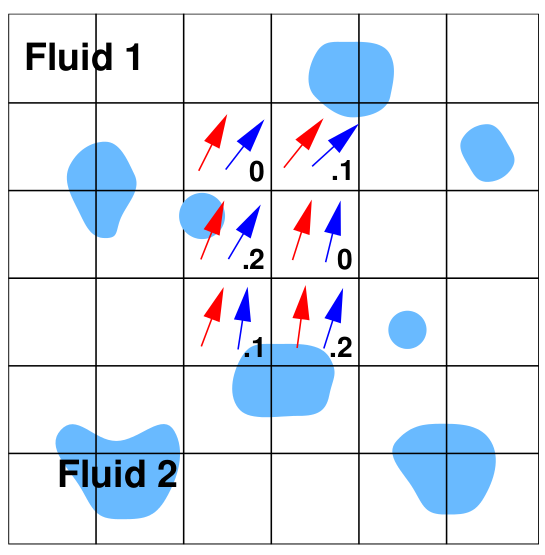
\includegraphics[width=0.4\linewidth]{eulerian}
\end{figure}
}

\only<2>{

\begin{itemize}
\item Continuity equation
\end{itemize}
\begin{equation}
\nabla\cdot\overline{U} =0
\end{equation}
\begin{equation}
\overline{U} =\alpha_a\overline{U}_a+\alpha_b\overline{U}_b
\end{equation}
\begin{itemize}
\item $\alpha_a$ equation (Weller (2002))
\end{itemize}
\begin{equation}
\frac{\partial\alpha_{a}}{\partial t}+ \nabla. (\overline{U}\alpha_{a})+\nabla. (\overline{U_r}\alpha_{a}(1-\alpha_{a}))=0
\end{equation}
\begin{itemize}
\item Momentum equation
\end{itemize}
\begin{equation}
\frac{\partial\alpha_\phi\overline{U}_\phi}{\partial t}+\nabla\cdot(\alpha_\phi\overline{U}_\phi\overline{U}_\phi)+\nabla\cdot (\alpha_\phi\overline{R}_\phi^{eff}) = -\frac{\alpha_\phi}{\rho_\phi}\nabla\overline{p}+\alpha_\phi g+\frac{\overline{M}_\phi}{\rho_\phi}
\label{eqn:eqn2.5}
\end{equation}
}
\only<3>{
\begin{itemize}
\item Inter-phase momentum transfer
\end{itemize}
\begin{equation}
\overline{M_a}=\overline{F}_d+\overline{F}_l+\overline{F}_{\nu m}
\label{eqn:eqn2.6}
\end{equation}
\begin{figure}
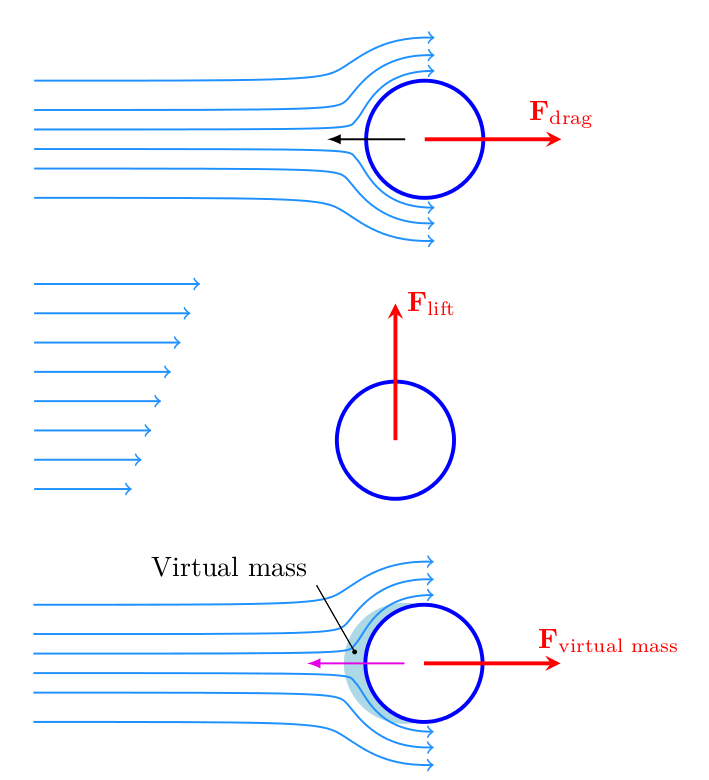
\includegraphics[width=0.4\linewidth]{exchange}
\end{figure}
}

\only<4>{
\begin{itemize}
\item Drag force: Schiller-Nauman (1935) model 
\end{itemize}
\begin{equation}
\overline{F}_d = \alpha C_d \frac{3}{4} \rho_b d_a \vert U_r \vert U_r
\label{eqn:eqn2.7}
\end{equation}

\begin{itemize}
\item Lift force
\end{itemize}
\begin{equation}
\overline{F}_l = 0
\label{eqn:eqn2.8}
\end{equation}

\begin{itemize}
\item Added mass force: $C_{\nu m} = 0.5 $
\end{itemize}
\begin{equation}
\overline{F}_{\nu m} = \alpha C_{\nu m} \rho_b (\frac{D_b U_b}{Dt}-\frac{D_a U_a}{Dt})
\label{eqn:eqn2.9} 
\end{equation}

}

\end{frame}


\subsection{Population balance model}

\begin{frame}{F. Kerdouss et al. (2006)}

\begin{equation} 
\frac{\partial n}{\partial t}+\nabla.({\textbf{U}_G}n) = S_{br}-S_{co} 
\end{equation}

\pause


\begin{equation}
S_{br} = C_{br} n (\frac{n u_t}{d}) exp (-\frac{We_{cr}}{We})\sqrt{1-\frac{We_{cr}}{We}}
\end{equation}

\pause

\begin{equation}
S_{co} = C_{co}\frac{n^2 u_t {D}^2}{1-\alpha_{G}^{1/3}}
\end{equation} 

\pause

\begin{equation}
u_t = \sqrt{2k}
\end{equation}

\pause

\begin{equation} 
\boxed{d = {\bigg[ \frac{6\alpha_{G}}{n{\pi}} \bigg]}^{\frac{1}{3}} } 
\end{equation} 
 
  
\end{frame}



\subsection{Turbulence two phase model }

\begin{frame}{kEpsilon model}


\begin{equation}
\frac{\partial}{\partial t} (\alpha_c k)+\nabla. (\alpha_c \textbf{U}_c k) = \nabla. (\alpha_c \frac{\nu_c^{T}}{\sigma_k} \nabla k)+\alpha_c G - \alpha_c \epsilon +\cancelto{0}{\alpha_c {\prod}_k^{dis}}+\cancelto{0}{\alpha_c {\prod}_k^i} 
\end{equation}


\begin{equation}
\frac{\partial}{\partial t} (\alpha_c \epsilon)+\nabla. (\alpha_c \textbf{U}_c \epsilon) = \nabla. (\alpha_c \frac{\nu_c^{T}}{\sigma_\epsilon} \nabla \epsilon)+ \alpha_c \frac{\epsilon}{k}(C_1G-C_2\epsilon)+\cancelto{0}{\alpha_c {\prod}_\epsilon^{dis}}+\cancelto{0}{\alpha_c {\prod}_\epsilon^i}  
\end{equation}

\begin{equation}
G = 2{\nu_c}^{eff} \big[ \nabla \textbf{U}_c.\textit{dev} (\nabla+{(\nabla \textbf{U}_c)}^T) \big]
\end{equation}

\begin{equation}
\nu_c^{t}= C_\mu \frac{k^2}{\epsilon}
\end{equation}

\end{frame}

\begin{frame}{kEpsilon model}

\begin{itemize}
  \item Richard T. Lahey Jr. 2005 
\end{itemize}


\begin{equation}
{\prod}_k^i= \frac{k}{C_{\epsilon_2} \epsilon} {\prod}_\epsilon^i  = C_p \big[ 1+C_D^{\frac{4}{3}} \big] \alpha_c \frac{|\textbf{U}_r|^3}{d_b}
\end{equation} 

\begin{equation}
{\prod}_k^{dis} = {\prod}_\epsilon^{dis} =0
\end{equation}

\begin{equation}
\nu_c^{t}= C_\mu \frac{k^2}{\epsilon}+0.6 \alpha_c d_b |\textbf{U}_r|
\end{equation}

\end{frame}




\section{Ranade's Bubble Column}

\begin{frame}{Bubble column}

  \begin{figure}
  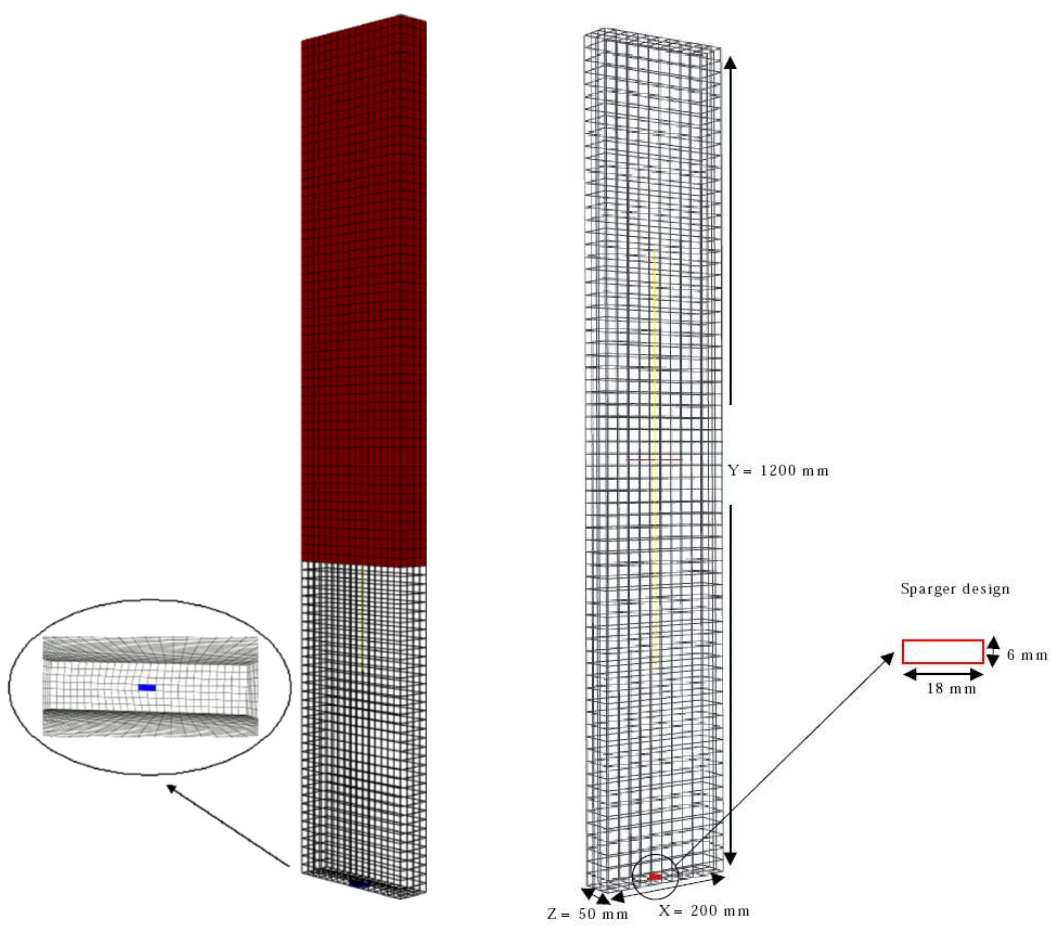
\includegraphics[width=0.3\linewidth]{geometry.png}
  \caption {Ranade bubble column}
  \end{figure}   
\end{frame}

\begin{frame}{Simulation pre-processing}
\begin{itemize}
\only<1>{
\item Dimensions: $0.2 \times 1.2 \times 0.05 $ m

  \begin{figure}
  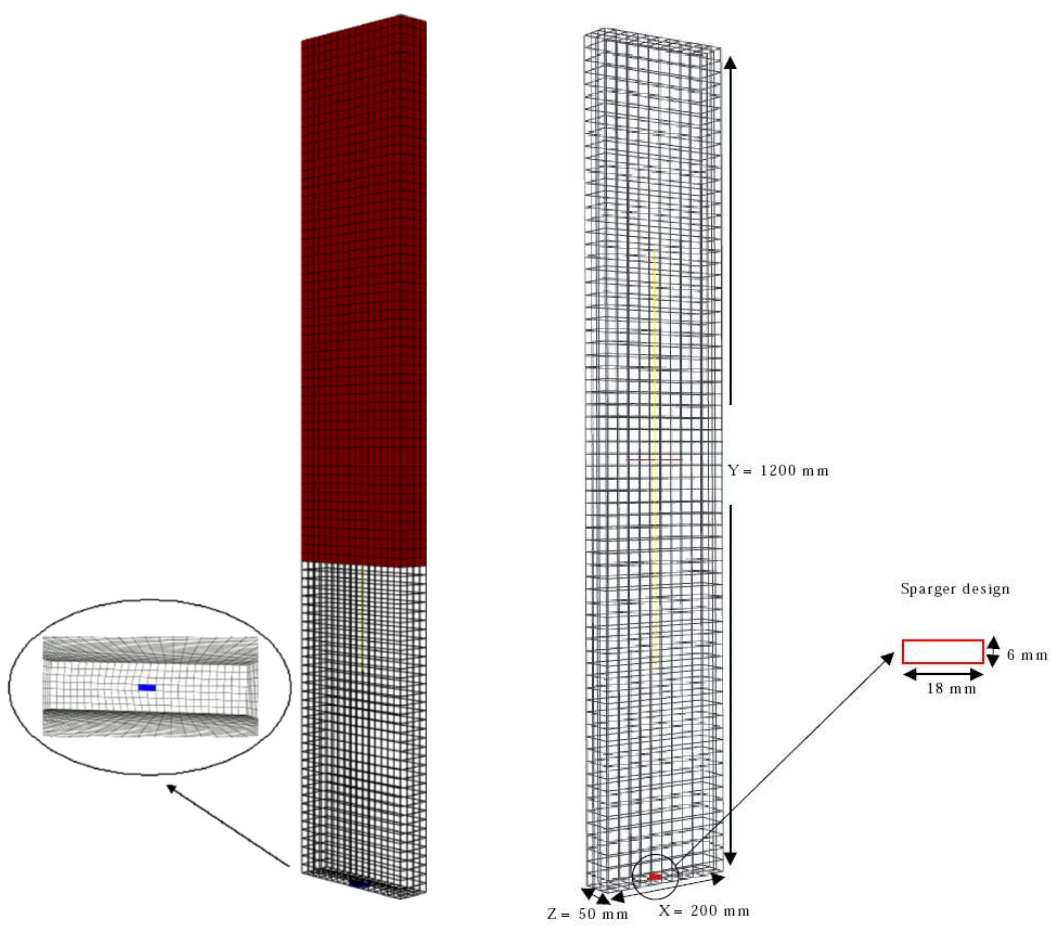
\includegraphics[width=0.3\linewidth]{geometry.png}

  \end{figure} 
  }
  
\only<2>{
\item Number of mesh: $6144$
  \begin{figure}
  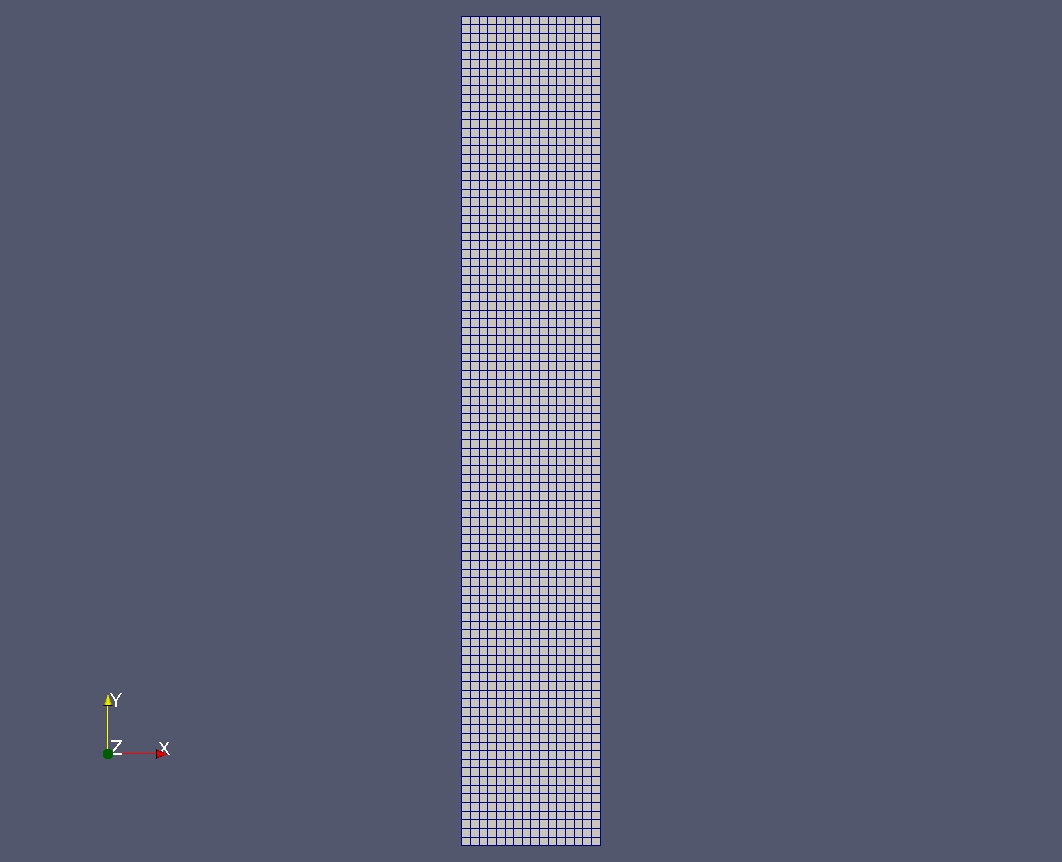
\includegraphics[width=0.5\linewidth]{mesh.jpg}
  \end{figure} 
}

\only<3>{

\item Perforated section: $18\times6$ $mm$
  \begin{figure}
  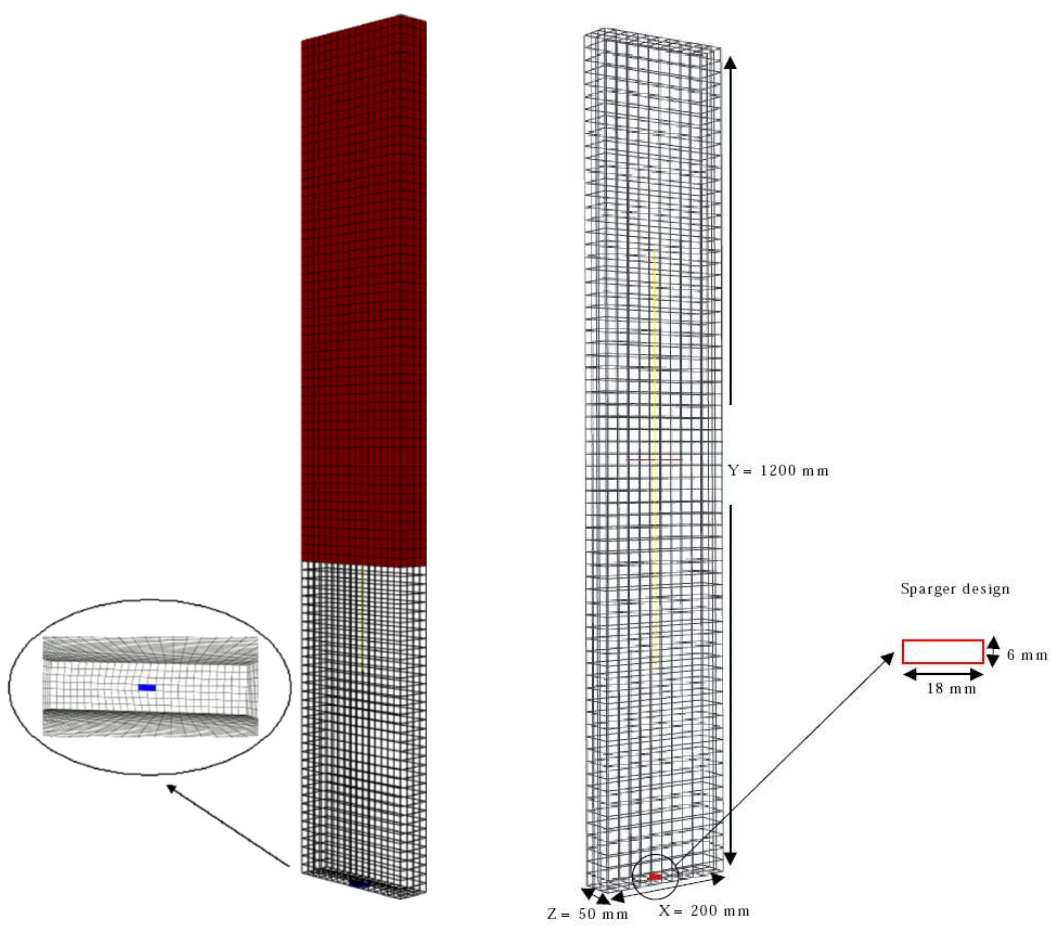
\includegraphics[width=0.3\linewidth]{geometry.png}
  \end{figure} 
}

\only<5>{ 
\item Gas inlet velocity: $U_{d,in}=0.14$ $m/s$
  \begin{figure}
  \includegraphics[width=0.5\linewidth]{Ua.jpg}
  \end{figure} 
}

\only<4>{
\item Liquid height in column: $0.45$ $m$ out of $1.2$ $m$
  \begin{figure}
  \includegraphics[width=0.5\linewidth]{BCu.jpg}
  \end{figure}
}
\only<6>{
\item $n=15286624$ $m^{-3}$, for $d_{sm}=5mm$, $\boxed{n =  \frac{6\alpha_{G}}{d^3{\pi}}}$ 
}
\only<7>{


\item Turbulent or Laminar ???


\begin{block}{1st Simulatiuon type}
\begin{center}
Laminar
\end{center}
\end{block}

\begin{block}{2nd Simulatiuon type}
\begin{center}
Turbulent
\end{center}
\end{block}


}
\end{itemize}
\end{frame}


\section{Simulation and Results}

% Placing a * after \section means it will not show in the
% outline or table of contents.
%%%%%%%%%%%%%%%%%%%%%%%%%%%%%%%%%%%%%%%%%%%%%%%%%%%%%%%%%%%%%%%%%%%%%%%%%%%%%%%%%%%%%%%%%%%%%%%%%%%%%%%%
\begin{frame}{Validation (Laminar)}

\begin{figure}
\includegraphics[width=0.6\linewidth]{laminar}
\caption {At $Y=37cm$ from bottom for \textbf{laminar}}
\end{figure}

\end{frame}

\begin{frame}{Gas volume fraction (laminar)}
  \includemovie[poster, text=(\textbf{PLAY}), mouse,repeat]{\linewidth}{0.6\linewidth}{alphaNoturb.mpg} 
\end{frame} 

\begin{frame}{Gas velocity (laminar)}
  \includemovie[poster, text=(\textbf{PLAY}), mouse, repeat]{\linewidth}{0.6\linewidth}{UairNoturb.mpg}
\end{frame}

\begin{frame}{Bubble size distribution (laminar)}
  \includemovie[poster, text=(\textbf{PLAY}), mouse, repeat]{\linewidth}{0.6\linewidth}{dairNoturb.mpg}
\end{frame}


%%%%%%%%%%%%%%%%%%%%%%%%%%%%%%%%%%%%%%%%%%%%%%%%%%%%%%%%%%%%%%%%%%%%%%%%%%%%%%%%%%%%%%%%%%%%%%%%%%%%%%%%
%%%%%%%%%%%%%%%%%%%%%%%%%%%%%%%%%%%%%%%%%%%%%%%%%%%%%%%%%%%%%%%%%%%%%%%%%%%%%%%%%%%%%%%%%%%%%%%%%%%%%%%%
\begin{frame}{Validation (kEpsilon)}


\only<1>{
\begin{itemize}
  \item kEpsilon model
\end{itemize}

\begin{equation}
{\prod}_k^i= {\prod}_\epsilon^i  = N. C
\end{equation} 

\begin{equation}
{\prod}_k^{dis} = {\prod}_\epsilon^{dis} = N. C
\end{equation}

\begin{equation}
\nu_c^{T}= C_\mu \frac{k^2}{\epsilon}
\end{equation}
}


\only<2>{
\begin{figure}
\includegraphics[width=0.6\linewidth]{KEp}
\caption {At $Y=37cm$ from bottom for \textbf{kEpsilon}}
\end{figure}
} 
\end{frame}


\begin{frame}{Gas volume fraction (kEpsilon)}
  \includemovie[poster, text=(\textbf{PLAY}), mouse,repeat]{\linewidth}{0.6\linewidth}{alphakEpsilon.mpg}
\end{frame}

\begin{frame}{Gas velocity (kEpsilon)}
  \includemovie[poster, text=(\textbf{PLAY}), mouse, repeat]{\linewidth}{0.6\linewidth}{UairkEpsilon.mpg}
\end{frame}

\begin{frame}{Bubble size distribution (kEpsilon)}
   \includemovie[poster, text=(\textbf{PLAY}), mouse, repeat]{\linewidth}{0.6\linewidth}{dairkEpsilon.mpg}
\end{frame}


%%%%%%%%%%%%%%%%%%%%%%%%%%%%%%%%%%%%%%%%%%%%%%%%%%%%%%%%%%%%%%%%%%%%%%%%%%%%%%%%%%%%%%%%%%%%%%%%%%%%%%%%
%%%%%%%%%%%%%%%%%%%%%%%%%%%%%%%%%%%%%%%%%%%%%%%%%%%%%%%%%%%%%%%%%%%%%%%%%%%%%%%%%%%%%%%%%%%%%%%%%%%%%%%%
\begin{frame}{Validation (LaheykEpsilon)}


\only<1>{
\begin{itemize}
  \item Richard T. Lahey Jr. 2005 
\end{itemize}


\begin{equation}
{\prod}_k^i= \frac{k}{C_{\epsilon_2} \epsilon} {\prod}_\epsilon^i  = C_p \big[ 1+C_D^{\frac{4}{3}} \big] \alpha_c \frac{|\textbf{U}_r|^3}{d_b}
\end{equation} 

\begin{equation}
{\prod}_k^{dis} = {\prod}_\epsilon^{dis} =0
\end{equation}

\begin{equation}
\nu_c^{T}= C_\mu \frac{k^2}{\epsilon}+0.6 \alpha_c d_b |\textbf{U}_r|
\end{equation}
}


\only<2>{
\begin{figure}
\includegraphics[width=0.6\linewidth]{LaheyKEp}
\caption {At $Y=37cm$ from bottom for \textbf{LaheyKEp}}
\end{figure}
} 

\end{frame}

\begin{frame}{Gas volume fraction (LaheyKEpsilon)}
   \includemovie[poster, text=(\textbf{PLAY}), mouse,repeat]{\linewidth}{0.6\linewidth}{alphaLahey.mpg}
\end{frame}

\begin{frame}{Gas velocity (LaheyKEpsilon)}
   \includemovie[poster, text=(\textbf{PLAY}), mouse, repeat]{\linewidth}{0.6\linewidth}{UairLahey.mpg}
\end{frame}

\begin{frame}{Bubble size distribution (LaheyKEpsilon)}
   \includemovie[poster, text=(\textbf{PLAY}), mouse, repeat]{\linewidth}{0.6\linewidth}{dairLahey.mpg}
\end{frame}



%%%%%%%%%%%%%%%%%%%%%%%%%%%%%%%%%%%%%%%%%%%%%%%%%%%%%%%%%%%%%%%%%%%%%%%%%%%%%%%%%%%%%%%%%%%%%%%%%%%%%%%%




\end{document}
